\documentclass[TFG.tex]{subfiles}

\begin{document}


%\hyphenation{equi-va-len-cia}\hyphenation{pro-pie-dad}\hyphenation{res-pec-ti-va-men-te}\hyphenation{sub-es-pa-cio}
\chapter{Representaciones lineales}

La existencia (o no existencia) de representaciones lineales fieles de los grupos de trenzas fue uno de los mayores problemas del campo. Este problema fue por primera vez resuelto por Bigelow \cite{Bigelow} y Krammer \cite{Krammer} en el año 2000, mediante la conocida como \emph{representación LKB}. Además de esta representación existen otras, como la representación de Burau, con la cual empezaremos este capítulo.

\section{Representación de Burau}

\subsection{Definición a partir de espacios recubridores}

Consideremos el disco agujereado $n$ veces $\D_n$ con un punto base $d_0\in\D_n$. 
\begin{defi}
Para cada lazo $\alpha$ basado en $d_0$ denominamos \emph{índice total}  a la suma de los índices (número de vueltas) de $\alpha$ con respecto a cada agujero y lo denotamos $\phi\alpha$. Esto es, si un $\alpha$ está representado en $F_n$ por $\prod_{i=1}^n x_i^{m_i}$, entonces 
\[
\phi\alpha=\sum_{i=1}^nm_i.
\]
\end{defi}

Se observa que $\phi$ es un homomorfismo de grupos $\phi:\pi_1(\D_n)\to\Z$ al ser el índice total un invariante homotópico. Sea $\tilde{\D}_n$ el espacio recubridor correspondiente a $\ker\phi$. Vamos a describir geométricamente este espacio recubridor (ver Figura \ref{recubrimiento}). 

%si es invariante homotópico también lo será por homeomorfismo

Para visualizarlo mejor, vamos a agrandar los agujeros de modo que se conviertan en bolas abiertas y llamamos a este nuevo espacio $X$. Dibujamos segmentos $A_1,\dots, A_n$ desde el centro de las bolas hasta el borde del disco. Cortamos $X$ a lo largo de estos segmentos, de modo que obtenemos dos copias disjuntas $A_i^+$ y $A_i^-$ de cada $A_i$. Llamamos a este espacio $X^*$. Sean $h_i:A_i^+\to A_i^-$ homeomorfismos y tomamos una cantidad numerable de copias $X^*_j$ de $X^*$. Para cada $j$ sea $g_j:X^*_j\to X^*$ un homeomorfismo. El espacio $\tilde{X}$ se define como la unión disjunta de los $X^*_j$ identificando $A_i^+\subseteq X^*_j$ con $A_i^-\subseteq X^*_{j+1}$ mediante $g_{j+1}^{-1}h_ig_j$.

%Se idenfitica A_i^+ con la imagen mediante la aplicación esa

\begin{figure}[h!]
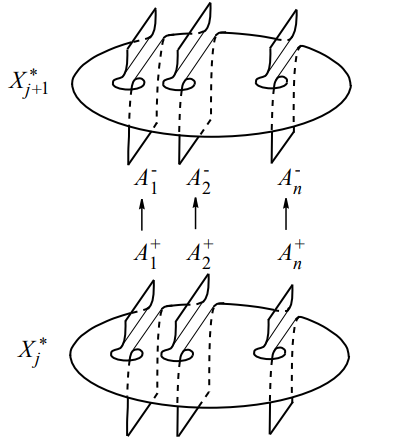
\includegraphics[scale=0.6]{Imagenes/recubrimiento}
\caption{Dos hojas del espacio recubridor $\tilde{X}$.}\label{recubrimiento}
\end{figure}

El hecho de que este sea el recubrimiento correspondiente a $\ker\phi$ se debe a que, fijada una preimagen $\tilde{d}_0\in\tilde{X}$ preimagen de $d_0$, un lazo en $d_0$ se levanta a un lazo en $\tilde{d}_0$ si y solo si su índice total es nulo, pues para cada vuelta positiva sube un nivel en el recubrimiento y para cada vuelta negativa lo baja, así que para acabar de nuevo en $\tilde{d}_0$ deberá subir tantas veces como baja, es decir, que el número total de vueltas sea nulo.

Hay una acción natural de $\Z$ en $\tilde{X}$ como transformación del recubrimiento dada por $X^*_j\ni x\mapsto g_{j+n}^{-1}g_jx$ para cada $n\in\Z$. Esta acción se puede interpretar como cambiar el punto $x$ de nivel. Además, la acción es claramente libre y el espacio de órbitas $\tilde{X}/\Z$ es $X$, por lo que el espacio recubridor es regular.


%PODRÍA DEFINIRLO ASÍ QUE ES MÁS SENCILLO EN LUGAR DE DEFINIRLO A PARTIR DE LAS TRANSFORMACIONES DE DECK QUE EMPIEZA COGIENDO AUTOMORFISMOS SOBRE LAS FIBRAS

%el espacio recubridor retrae con deformación sobre Z copias de n cuerdas con los extremos unidos a un mismo punto.

POSIBLEMENTE CAMBIAR LA NOTACIÓN ESTRELLA POR LA DE CLASE DE EQUIVALENCIA

Vamos a ver cómo definir la representación de Burau. Sea $\beta\in B_n$ inducida por un automorfismo $h$ de $\D_n$ fijando el borde, lo cual vamos a denotarlo $\beta=h_*$. Entonces, para cualquier lazo $\gamma$ en $\D_n$ se tiene que $\phi(h\gamma)=\gamma$, de modo que $h$ se levanta a unz equivalencia de homotopía \cite{Hatcher} $\tilde{h}$ de $\tilde{\D}_n$ que fija el borde. Pasando a la homología, esto nos da un automorfismo de $H_1(\tilde{\D}_n)$. Si $h'$ es cualquier otro automorfismo con $h'_*=\beta$, entonces $h_*^{-1}h'_*=1$, así que como la aplicación inducida por el recubrimiento $\pi_1(\tilde{\D}_n)\to\pi_1(\D_n)$ es inyectiva \cite{Hatcher} tenemos que $\tilde{h}_*^{-1}\tilde{h}'_*=1$ como aplicación en $\pi_1(\tilde{\D}_n)$. Pasando a homología, esto nos da $\tilde{h}'_*-\tilde{h}_*=1$ como aplicación en $H_1(\tilde{\D}_n)$. 

%EL SEGUNDO PASO A HOMOLOGÍA SE HACE ABELIANIZANDO CON HUREWICZ

%AQUÍ TENGO UNA PREGUNTA COMENTADA EN EL TEX
%¿Se puede levantar siempre el automorfismo? Supongo que sí, porque $p:X->Dn, h:Dn->Dn$, entonces cojo para cada fibra $p^{-1}hp: X -> X$. Como en los segmentos coincide para cada fibra, se extiende a todo X. 


\begin{defi}
Sea el homomorfismo $\psi_r:B_n\to GL(H_1(\tilde{\D}_n))$ dado por $\psi_r(\beta)=\tilde{h}_*$. Esta aplicación está bien definida por las observaciones anteriores y es lo que se conoce como \emph{representación de Burau reducida} de $B_n$.
\end{defi}

Se llama \emph{reducida} porque existe una representación $n$-dimensional de la cual la forma reducida es un sumando irreducible. Esta mencionada representación $n$-dimensional puede encontrarse en \cite{thesis}. Como veremos con la siguiente proposición, la representación que hemos dado es $n-1$-dimensional.

¿SUMANDO IRREDUCIBLE QUÉ SIGNIFICA? ¿COMO SUMA DIRECTA?

\begin{prop}
$H_1(\tilde{\D}_n)$ es un módulo libre de rango $n-1$ sobre $\Z[t,t^{-1}]$.
\end{prop}
\begin{dem}
En esta prueba quiero saber qué significa cuando coge el generador, si es un espacio topológico
\end{dem}


%Lo de que se corresponda al ker es como cuando en Hatcher hace corresponder un espacio recubridor de S1vS1 a cada grupo libre generado con combinaciones de los lazos ab. Como explica Hatcher, se hace cogiendo la imagen del homomorfismo inducido por el recubrimiento en el grupo fundamental del recubrimiento fijando un punto base preimagen del punto base de X. El subgrupo generado por esta imagen en pi(X,x0) es el que se corresponde con el recubrimiento. En este caso, fijada una preimagen de d0, los lazos en d0 son los que tienen total winding number 0 porque cada vez que hacen un giro bajan o suben de nivel, por lo que para volver a d0 tienen que subir lo mismo que bajan

%el homomorfismo inducido por el recubrimiento en los grupos fundamentales es siempre inyectivo (Hatcher)

%Over a commutative ring R, more care is needed: a matrix over R is invertible if and only if its determinant is a unit in R, that is, if its determinant is invertible in R. Therefore, GL(n, R) may be defined as the group of matrices whose determinants are units.
\subsection{Expresión matricial}
Con las últimas observaciones del apartado anterior podemos obtener fácilmente la expresión matricial de la representación de Burau. Como la Figura \ref{representacion} muestra, la acción de $\sigma_i$ sobre $H_1(\tilde{X})$ viene dada por
MUY PROBABLEMENTE TENGA QUE CAMBIAR TANTO EL DIBUJO COMO LA REPRESENTACIÓN PORQUE NO ENTIENDO NADA
\[
\psi_r\sigma_i(v_j)=\begin{cases}
v_j+tv_{j+1} & j=i-1,\\
-tv_j & j=i,\\
v_{j-1}+v_j,\\
v_j & c.c.
\end{cases}
\]

Por lo tanto, las matrices para la representación con respecto a la base $\{v_1,\dots, v_n\}$ son
\[
\psi_r(\sigma_1)=\begin{pmatrix}
-t & 1 & \\
0 & 1 & \\
& & I_{n-3}
\end{pmatrix},\psi_r(\sigma_i )=\begin{pmatrix}
I_{i-2} & & &\\
& 1 & 0 & 0 & \\
& t & -t & 1 & \\
& 0 & 0 & 1 & \\
& & & & I_{n-i-2}  
\end{pmatrix}, \psi_r(\sigma_{n-1})=\begin{pmatrix}
I_{n-3} & &\\
1 & 0 & \\
t & -t & 
\end{pmatrix}.
\]

Se puede comprobar directamente que las matrices anteriores satisfacen las relaciones de la presentación \ref{presentacion}. Un hecho interesante de esta representación es que se sabe que es fiel para $n\leq 3$ \cite{Birman} y que no es fiel para $n\geq 5$ \cite{Bil}\cite{LP}, pero el caso $n=4$ sigue siendo un problema abierto.

\section{Representación LKB}
%Buscar por qué LKB, supongo que Krammer y Bigelow, pero la L no sé. Alomejor Luis Paris me da una pista.
Siguiendo \cite{Krammer}, denotamos $Ref_n$ al conjunto de pares de enteros $(i,j)$ tales que $1\leq i<j\leq n$. Claramente, el cardinal de $Ref_n$ es $\dfrac{n(n-1)}{2}$.

Sea $R$ un anillo conmutativo con unidad y $q,t\in R$ dos elementos invertibles. Sea $V=\oplus_{s\in Ref_n}Rx_s$ el $R$-módulo libre de rango $\dfrac{n(n-1)}{2}$ con base $\{x_s\}_{s\in Ref_n}$. Krammer define una acción $R$-lineal de $B_n$ sobre $V$ como sigue


EL RANGO DE UN MÓDULO LIBRE NO ESTÁ ÚNICAMENTE DEFINIDO, ¿TIENE SENTIDO?
\begin{equation}\label{LKB}
\sigma_k(x_{i,j})=\begin{cases}
x_{i,j} & \textit{si }(k<i)\text{ o }(j<k),\\
x_{i-1,k}+(1-q)x_{i,j} & \text{si } (k=i-1),\\
tq(q-1)x_{i,i+1}+qx_{i+1,j} & \text{si }(k=i<j-1),\\
tq^2x_{i,j} & \text{si }k=i=j-1,\\
x_{i,j}+tq^{k-i}(q-1)^2x_{k,k+1} & \text{si }(i<k<j-1),\\
x_{i,j-1}+tq^{j-1}(q-1)x_{j-1,j} & \text{si }(i<k=j-1),\\
(1-q)x_{i,j}+qx_{i,j+1} & \text{si }(k=j),
\end{cases}
\end{equation}
donde $1\leq i<j\leq n$ y $k=1,\dots, n-1$. Que la acción de $\sigma_k$ es invertible y que se cumplen las relaciones de \ref{presentacion} se verifica mediante cálculo directo. Esta es la conocida como \emph{representación LKB} o \emph{representación de Krammer} de $B_n$.


%Para dar la matriz habría primero que fijar un orden en Ref y ya está
\begin{teorema}
Sea $R=\R[t^{\pm 1}]$ y $0<q<1$. Entonces, la representación $B_n\to Aut(V)$ es fiel para todo $n\geq 1$.
\end{teorema}

La prueba de este teorema se encuentra en \cite{Krammer}.

%Rango=número de generadores libres

\subsection{Representación de Bigelow}
Existe un caso particular de la representación LKB encontrada independiente por Bigelow \cite{Bil}, la cual se puede obtener usando $R=\Z[q^{\pm 1},t^{\pm 1}]$. La ventaja de esta representación es que tiene una interpretación geométrica mucho más clara, como veremos a continuación.

Consideremos $C=M_2(\D_n)/\Sigma_2$. Aquí, $\Sigma_2$ actúa sobre $M_2(\D_n)$ enviando $(x,y)$ a $(y,x)$. Se denotarán los puntos de $C$ como $\{x,y\}$ ya que al actuar $\Sigma_2$ no importa el orden. La proyección $M_2(\D_n)\to C$ que lleva $(x,y)$ a $\{x,y\}$ es claramente un recubrimiento de dos hojas. Sean $d_0$ y $d_0'$ dos puntos de $\partial\D_n$ los bastante cercano entre sí. Tomamos $c_0=\{d_0,d_0'\}$ como punto base de $C$.

%Es sobreyectiva y continua porque la preimagen de un abierto es unión de dos abiertos simétricos y disjuntos porque no está la diagonal

Sea $\alpha:[0,1]\to C$ un camino basado $c_0$. Este camino se puede levantar relativamente a $(d_0,d_0')$ como un par de caminos de la forma $(\alpha_1,\alpha_2)$, con$ \alpha_1,\alpha_2:[0,1]\to\D_n$, el primero basado en $d_0$ y el segundo en $d_0'$. Denotemos pues $\alpha(t)=\{\alpha_1(t),\alpha_2(t)\}$. Nótese que si $\alpha$ es un lazo entonces $\{\alpha_1(0),\alpha_2(0)\}=\{\alpha_1(1),\alpha_2(1)\}=\{d_0,d_0'\}$. Por lo tanto, o bien $\alpha_1$ y $\alpha_2$ son ambos lazos o bien su concatenación forma un lazo. Ambos casos se observan en la Figura \ref{loop}. 

\begin{figure}[h!]
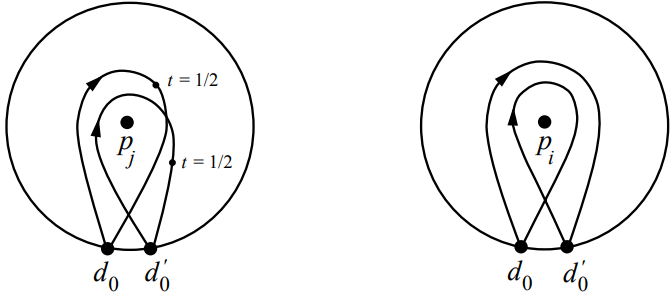
\includegraphics[scale=0.6]{Imagenes/loop}
\caption{A la izquierda, un lazo en $C$ que surge cuando los dos caminos originales son lazos (el parámetro $t$ muestra cómo está parametrizado el lazo). A la derecha, la concatenación de los dos lazos originales da lugar a un lazo en $C$.}\label{loop}
\end{figure}

%en la figura se ve que se cortan, pero basta que no se corten para el mismo valor de t

Si $\alpha_1$ y $\alpha_2$ son caminos en $\D_n$ con $\alpha_1(t)\neq\alpha_2(t)$ para todo $t\in[0,1]$, entonces $(\alpha_1,\alpha_2)$ es un camino en $M_2(\D_n)$. La imagen de este camino mediante la proyección $M_2(\D_n)\to C$ se denota $\{\alpha_1,\alpha_2\}$.

Sea $\alpha:I\to C$ un representante de un elemento en $\pi_1(C)$. Se definen las aplicaciones $a,b:\pi_1(C)\to\Z$ como sigue: si $\alpha_1$ y $\alpha_2$ son ambos lazos, entonces $a(\alpha)$ es la suma de los índices totales de $\alpha_1$ y $\alpha_2$. Si no son ambos lazos, entonces $a(\alpha)$ es el índice total del lazo $\alpha_1\alpha_2$. La aplicación $b$ está definida en primer lugar componiendo $I\ni t\mapsto \dfrac{(\alpha_1(t)-\alpha_2(t))}{|\alpha_1(t)-\alpha_2(t)|}\in S^1$ con la proyección $S^1\to \R P^1$ para obtener un lazo en $\R P^1$. El correspondiente elemento de $H_1(\R P^1)\cong\Z$ es $b(\alpha)$. Por tanto, $a$ mide la cantidad de veces que los lazos $\alpha_1$ y $\alpha_2$ envuelven a los agujeros, mientras que $b$ mide las veces que un lazo envuelve al otro.

SI RP ES HOMEOMORFO A S1, ¿PARA QUÉ PROYECTAR? 

LO DE B IGUAL TENDRÍA QUE VERLO CON MÁS CLARIDAD

Sea $\langle q,t\rangle$ el grupo libre abeliano  generado por $q$ y $t$. Se define la aplicación $\phi:\pi_1(C)\to\langle q,t\rangle$ mediante $\alpha\mapsto q^{a(\alpha)}t^{b(\alpha)}$. Por ejemplo, si en la Figura \ref{loop} denotamos al lazo de la izquierda $\gamma_1$ y al de la derecha $\gamma_2$, tenemos $\phi(\gamma_1)=q^2$ y $\phi(\gamma_2)=tq^2$. 

Sea $\tilde{C}\to C$ el espacio recubridor correspondiente a $\ker\phi$ y elijamos un levantamiento $\tilde{c}_0\in\tilde{C}$ de $c_0$. El grupo $\langle t,q\rangle$ actúa sobre $\tilde{C}$ como transformaciones del recubrimiento \cite{thesis}. Por tanto, el grupo de homología $H_2(\tilde{C})$ se convierte en un $\Z[q^{\pm 1},t^{\pm 1}]$-módulo \cite{nundam}.

Sea $h$ un automorfismo de $\D_n$ que fije el borde punto a punto. Entonces $h$ induce un automorfismo denotado igual $h:C\to C$ dado por $h(\{x,y\})=\{h(x),h(y)\}$. Es fácil comprobar que $h(c_0)=c_0$ y que la acción de $h$ en $H_1(C)$ conmuta con $\phi$. Por tanto, este homeomorfismo se levanta de forma única a una aplicación $\tilde{h}:\tilde{C}\to\tilde{C}$ que fija la fibra sobre $c_0$ punto a punto y conmuta con las transformaciones $q$ y $t$. Por tanto, $\tilde{h}$ induce un isomorfismo de $\Z[q^{\pm 1},t^{\pm 1}]$-módulos $\tilde{h}_*:H_2(\tilde{C})\to H_2(\tilde{C})$.

NO SÉ QUÉ SIGNIFICA AQUÍ QUE CONMUTE, PORQUE PUEDO HACER PHI DE H(ALPHA), PERO NO AL REVÉS

\begin{defi}
La representación $\kappa:B_n\to Aut(H_2(\tilde{C}))$ inducida por $h\to\tilde{h}_*$ se llama \emph{representación de Bigelow}.
\end{defi}

Este resultado se prueba en \cite{Bil}. También por \cite{Bil} podemos tomar una base $\{v_{i,j}\in H_2(\tilde{C})\}_{(i,j)\in Ref}$. Con esto, podemos establecer la equivalencia \cite{nundam} entre esta representación de la representación  \ref{LKB} como sigue:
\[
v_{i,j}=x_{i,j}+(1-q)\sum_{i<k<j}x_{k,j},\quad x_{i,j}=v_{i,j}+(q-1)\sum_{i<k<j}q^{k-i-1}v_{k,j}.
\]

%El punto base se fija porque está en el borde

\section{Solución al problema de la palabra}
¿SIMPLEMENTE MULTIPLICAR LAS MATRICES Y VER LO QUE SALE?

Una vez obtenida una representación lineal fiel, es inmediato resolver el problema de la palabra a partir de la expresión matricial: basta hacer el producto de las matrices que representan las letras de la palabra. Si el resultado de dicho producto es la matriz identidad, entonces la palabra es trivial y recíprocamente.

EN BURAU NO LO HE DICHO EXPLÍCITAMENTE, PERO ENTIENDO QUE LA MATRIZ DE LA INVERSA ES LA INVERSA DE LA MATRIZ

ALGO SOBRE LA EFICIENCIA DEL ALGORITMO

\begin{ej}
Vamos a ver un ejemplo de resolver el problema de la palabra con la representación de Burau para $n=3$, caso para el que sabemos que la representación es fiel. Para cualquier otra representación la mecánica es la misma. Consideremos la palabra $\sigma_1\sigma_1\sigma_2\sigma_1^{-1}\sigma_2^{-1}\sigma_1$. En este caso, tenemos las matrices
\[
\psi_r(\sigma_1)=\begin{pmatrix}
-t&1 \\
0 & 1
\end{pmatrix},\quad \psi_r(\sigma_2)=\begin{pmatrix}
1&0 \\
t&-t
\end{pmatrix}.
\]
Para este caso necesitaremos también las inversas
\[
\psi_r(\sigma_1^{-1})=\psi_r(\sigma_1)^{-1}=\begin{pmatrix}
-t^{-1}&t^{-1} \\
0&1
\end{pmatrix},\quad \psi_r(\sigma_2^{-1})=\psi_r(\sigma_2)^{-1}=\begin{pmatrix}
1&0 \\
1&-t^{-1}
\end{pmatrix}.
\]
Ahora, basta realizar el producto matricial
\[
\begin{pmatrix}
-t&1 \\
0 & 1
\end{pmatrix}
\begin{pmatrix}
-t&1 \\
0 & 1
\end{pmatrix}\begin{pmatrix}
1&0 \\
t&-t
\end{pmatrix}\begin{pmatrix}
-t^{-1}&t^{-1} \\
0&1
\end{pmatrix}\begin{pmatrix}
1&0 \\
1&-t^{-1}
\end{pmatrix}\begin{pmatrix}
-t&1 \\
0 & 1
\end{pmatrix}=
\]
\[
\begin{pmatrix}
(1-t)t^2& (1-t)^2-\frac{t^2+(1-t)t}{t^2}\\
t^2& (1-t)-\frac{1}{t}
\end{pmatrix}.
\]
Como la matriz no es la identidad, la palabra no representaba el elemento neutro.
\end{ej}

\end{document}
%https://arxiv.org/pdf/math/0006202.pdf
%http://ms.mcmaster.ca/~boden/students/Smeltzer-MSc.pdf
%Creo que el de encima y el de debajo son el mismo
% HE ESCRITO LO DE ESTA EN KRAMMER http://www.numdam.org/article/SB_1999-2000__42__389_0.pdf Aquí comenta cuándo la de Burau es fiel y cuándo no y quiénes lo probaron
%La de Krammer sí es faithful siempre
%LKB http://wrap.warwick.ac.uk/90207/1/WRAP_Theses_Coles_2017.pdf 

%Este tiene buena pinta http://go.owu.edu/~chjackso/Papers/thesis.pdf